\chapter{Introduction}

This introduction section will provide an overview of the sustainability crisis, outline the project's focus within the problem, and contextualize the following literature review.

\section{Sustainability Crisis in the Fashion Industry}
The fashion industry is a significant contributor to environmental degradation, second only to oil and mining. Waste and inefficiencies are endemic over the entire lifecycle. 
\subsection{Sourcing and Processing}
The problem starts from yarn production whether harvesting natural materials like cotton or the production of synthetic fibres. For example, cotton farming uses pesticides and fertilizers that pollute soil and water, leading to disasters like the Aral Sea shrinkage, while polyester production emits greenhouse gases and microplastics, harming marine life and human health. Furthermore, dyeing and finishing processes in textile manufacturing release harmful chemicals into water bodies, affecting aquatic ecosystems and human health. According to the Ellen MacArthur Foundation, the industry is responsible for approximately 10\% of global carbon emissions and is the second-largest consumer of the world's water supply.
\begin{figure} [H]
    \centering
    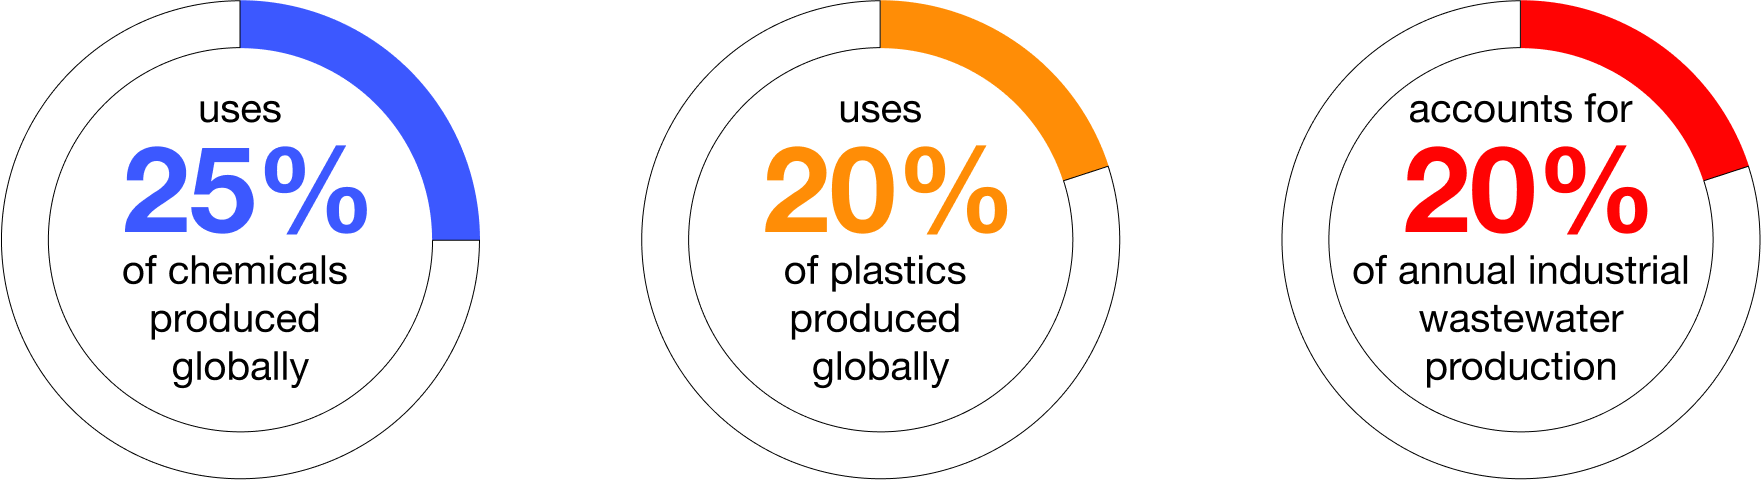
\includegraphics[width=0.8\textwidth]{Images/sourcing donuts.png}
    \caption{Fashion industry consumption metrics}
\end{figure}
\subsection{Overproduction and Overconsumption}
The fast fashion business model results in a relentless cycle of overproduction and overconsumption. Brands rapidly produce large quantities of low-cost, low-quality garments to chase ever-changing trends and induce consumer demand. Estimates suggest that by 2050, annual garment production will reach a staggering 814 billion garments, with a cumulative total of over 9.5 trillion garments produced from now until then. Social pressure to frequently update wardrobes undermines eco-conscious consumerism, fostering a throwaway culture, where clothing is discarded after only a few uses. During garment production, an average of approximately 15\% of fabric per garment is wasted during the cutting process. Thus, the resulting unsustainability is multi-dimensional: cut losses are often not recycled, unsold inventory is discarded, and consumers quickly dispose of their purchases. Pan describes this as a 'wicked problem' plagued by short product life cycles and excessive waste.

\section{Project Focus}
Within the fashion supply chain, this project focuses on the garment manufacturing stage and how to reduce waste both pre and post the point of sale. This is a question of material efficiency but also of what makes a garment desirable and why people might value it on an individual level. 

The project will explore the concept of 'zero waste patterns' and how they can be parameterised based on individual body measurements. The aim is to create designs that are both sustainable and desirable, increasing garment utility by recouping fabric cut loss. This will involve exploring the principles of zero waste pattern making, bespoke clothing, and garment utility, and how these concepts can be integrated into the design process. 

% The project will also investigate new tools that allow end-users to visualise the drape and fit of 2D patterns in 3D, enabling them to make more informed decisions about their clothing purchases.  DO WE ALSO WANT TO INCLUDE HERE HOW THE PROJECT WILL BE EVALUATED?